

\tikzset{every picture/.style={line width=0.75pt}} %set default line width to 0.75pt        

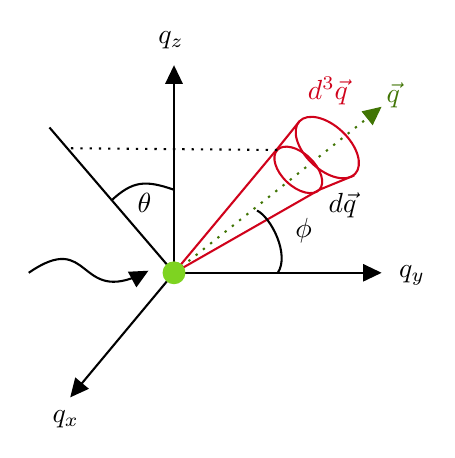
\begin{tikzpicture}[x=0.75pt,y=0.75pt,yscale=-1,xscale=1]
	%uncomment if require: \path (0,362); %set diagram left start at 0, and has height of 362
	
	%Straight Lines [id:da8075674552034334] 
	\draw    (270,180) -- (210,110) ;
	%Straight Lines [id:da1934453842044379] 
	\draw [color={rgb, 255:red, 65; green, 117; blue, 5 }  ,draw opacity=1 ] [dash pattern={on 0.84pt off 2.51pt}]  (270,180) -- (367.66,101.87) ;
	\draw [shift={(370,100)}, rotate = 141.34] [fill={rgb, 255:red, 65; green, 117; blue, 5 }  ,fill opacity=1 ][line width=0.08]  [draw opacity=0] (8.93,-4.29) -- (0,0) -- (8.93,4.29) -- cycle    ;
	%Straight Lines [id:da551977907100426] 
	\draw [color={rgb, 255:red, 208; green, 2; blue, 27 }  ,draw opacity=1 ]   (270,180) -- (340,140) ;
	%Straight Lines [id:da13834667273930523] 
	\draw [color={rgb, 255:red, 208; green, 2; blue, 27 }  ,draw opacity=1 ]   (270,180) -- (320,120) ;
	%Straight Lines [id:da575178064615293] 
	\draw    (270,180) -- (270,83) ;
	\draw [shift={(270,80)}, rotate = 90] [fill={rgb, 255:red, 0; green, 0; blue, 0 }  ][line width=0.08]  [draw opacity=0] (8.93,-4.29) -- (0,0) -- (8.93,4.29) -- cycle    ;
	%Straight Lines [id:da30763782233069703] 
	\draw    (270,180) -- (367,180) ;
	\draw [shift={(370,180)}, rotate = 180] [fill={rgb, 255:red, 0; green, 0; blue, 0 }  ][line width=0.08]  [draw opacity=0] (8.93,-4.29) -- (0,0) -- (8.93,4.29) -- cycle    ;
	%Straight Lines [id:da016368323591563816] 
	\draw    (270,180) -- (221.92,237.7) ;
	\draw [shift={(220,240)}, rotate = 309.81] [fill={rgb, 255:red, 0; green, 0; blue, 0 }  ][line width=0.08]  [draw opacity=0] (8.93,-4.29) -- (0,0) -- (8.93,4.29) -- cycle    ;
	%Curve Lines [id:da6672149281430028] 
	\draw    (200,180) .. controls (230.55,158.88) and (223.07,196.06) .. (255.12,180.32) ;
	\draw [shift={(257.67,179)}, rotate = 151.5] [fill={rgb, 255:red, 0; green, 0; blue, 0 }  ][line width=0.08]  [draw opacity=0] (8.93,-4.29) -- (0,0) -- (8.93,4.29) -- cycle    ;
	%Flowchart: Connector [id:dp12078467552802752] 
	\draw  [color={rgb, 255:red, 126; green, 211; blue, 33 }  ,draw opacity=1 ][fill={rgb, 255:red, 126; green, 211; blue, 33 }  ,fill opacity=1 ] (265,180) .. controls (265,177.24) and (267.24,175) .. (270,175) .. controls (272.76,175) and (275,177.24) .. (275,180) .. controls (275,182.76) and (272.76,185) .. (270,185) .. controls (267.24,185) and (265,182.76) .. (265,180) -- cycle ;
	%Shape: Ellipse [id:dp45046333760686075] 
	\draw  [color={rgb, 255:red, 208; green, 2; blue, 27 }  ,draw opacity=1 ] (319.75,120.83) .. controls (322.77,117.63) and (329.76,119.33) .. (335.35,124.63) .. controls (340.94,129.92) and (343.03,136.8) .. (340,140) .. controls (336.97,143.2) and (329.99,141.49) .. (324.4,136.2) .. controls (318.8,130.91) and (316.72,124.02) .. (319.75,120.83) -- cycle ;
	%Straight Lines [id:da9664046710126799] 
	\draw  [dash pattern={on 0.84pt off 2.51pt}]  (319.75,120.83) -- (220,120) ;
	%Curve Lines [id:da6106413145156059] 
	\draw    (310,150) .. controls (316.83,153.33) and (325.83,171.33) .. (320,180) ;
	%Curve Lines [id:da19983569644229238] 
	\draw    (240,145) .. controls (249.83,136) and (255.83,135) .. (270,140) ;
	%Shape: Ellipse [id:dp12574224384851007] 
	\draw  [color={rgb, 255:red, 208; green, 2; blue, 27 }  ,draw opacity=1 ] (330.45,106.98) .. controls (334.46,102.76) and (343.7,105.01) .. (351.1,112.01) .. controls (358.5,119.01) and (361.25,128.12) .. (357.25,132.35) .. controls (353.24,136.57) and (344,134.32) .. (336.6,127.32) .. controls (329.21,120.32) and (326.45,111.21) .. (330.45,106.98) -- cycle ;
	%Straight Lines [id:da8363641219417073] 
	\draw [color={rgb, 255:red, 208; green, 2; blue, 27 }  ,draw opacity=1 ]   (340,140) -- (356.87,133.07) ;
	%Straight Lines [id:da3377886983038795] 
	\draw [color={rgb, 255:red, 208; green, 2; blue, 27 }  ,draw opacity=1 ]   (320,120) -- (330.45,106.98) ;
	
	% Text Node
	\draw (261,62.4) node [anchor=north west][inner sep=0.75pt]    {$q_{z}$};
	% Text Node
	\draw (377,175) node [anchor=north west][inner sep=0.75pt]    {$q_{y}$};
	% Text Node
	\draw (210,245) node [anchor=north west][inner sep=0.75pt]    {$q_{x}$};
	% Text Node
	\draw (327,152.4) node [anchor=north west][inner sep=0.75pt]    {$\phi $};
	% Text Node
	\draw (251,140) node [anchor=north west][inner sep=0.75pt]    {$\theta $};
	% Text Node
	\draw (333,84) node [anchor=north west][inner sep=0.75pt]  [color={rgb, 255:red, 208; green, 2; blue, 27 }  ,opacity=1 ]  {$\text{d}^{3} \vec{q}$};
	% Text Node
	\draw (343,140) node [anchor=north west][inner sep=0.75pt]    {$\text{d}\vec{q}$};
	% Text Node
	\draw (371,87) node [anchor=north west][inner sep=0.75pt]  [color={rgb, 255:red, 65; green, 117; blue, 5 }  ,opacity=1 ]  {$\vec{q}$};
	
	
\end{tikzpicture}